\documentclass{article}
\usepackage{graphicx}
\graphicspath{ {./img} }
\begin{document}

\begin{center}
    \Large
    \textbf{3dViewer User's Guide}

    \vspace{0.5cm}

    \textit{By Exeggutor}

    \textit{and}

    \textit{Joseth Denese}

    \vspace{0.5cm}

    A primitive 3dViewer that loads up some coordinates and displays an object that user can view from different angles.
\end{center}

\pagebreak

\section{Features \& key interface elements}

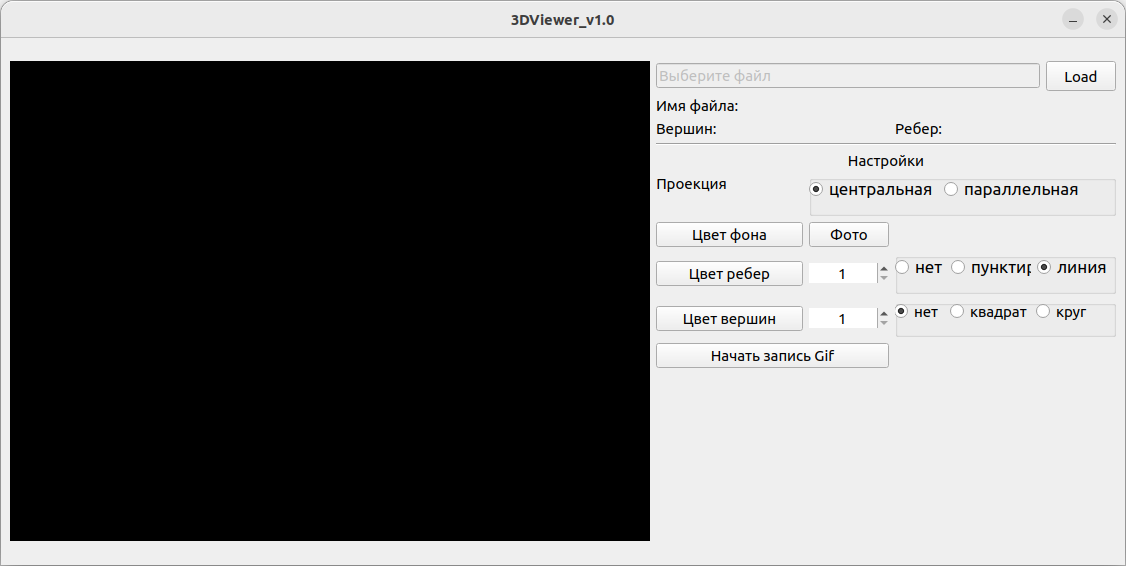
\includegraphics[width=10cm, keepaspectratio]{3dv_1}

\begin{enumerate}
    \item Left half of the app is taken by the 3d object render space
    \item On the top of the right half there is a loading zone
    \item In the middle there is an affine zone
    \item At the bottom there is the adjustment \& rendering zone
\end{enumerate}

\pagebreak

\section{Detailed explanation}
\subsection{Render space}

This is where you can see your loaded object and the results of your manipulations with it.

\subsection{Loading zone}

This is where you can load an \textit{.obj} file by pressing the \textbf{Load} button and selecting the file in the opened window.
If the file was successfully loaded, you'll be able to see file name, full file name and amount of nodes and edges the loaded object has.

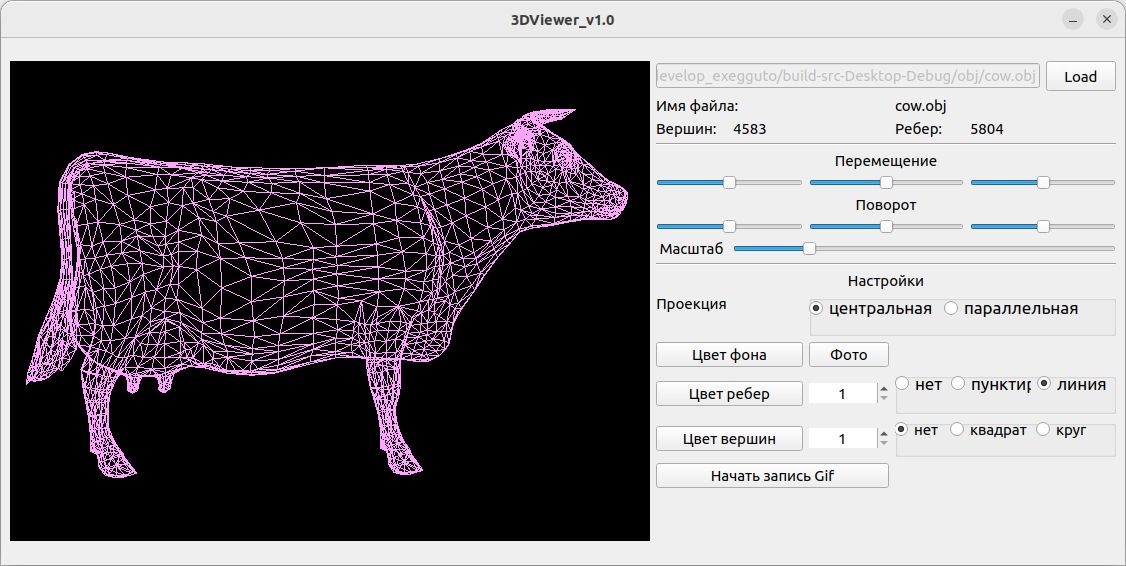
\includegraphics[width=10cm, keepaspectratio]{3dv_loading}

\subsection{Affine zone}

This is where you can adjust the object position (translate, rotate and scale) by moving the corresponding sliders.
Sliders are invisible until an \textit{.obj} file has been successfully loaded.
Moving any slider immediately re-renders the object on the render space.

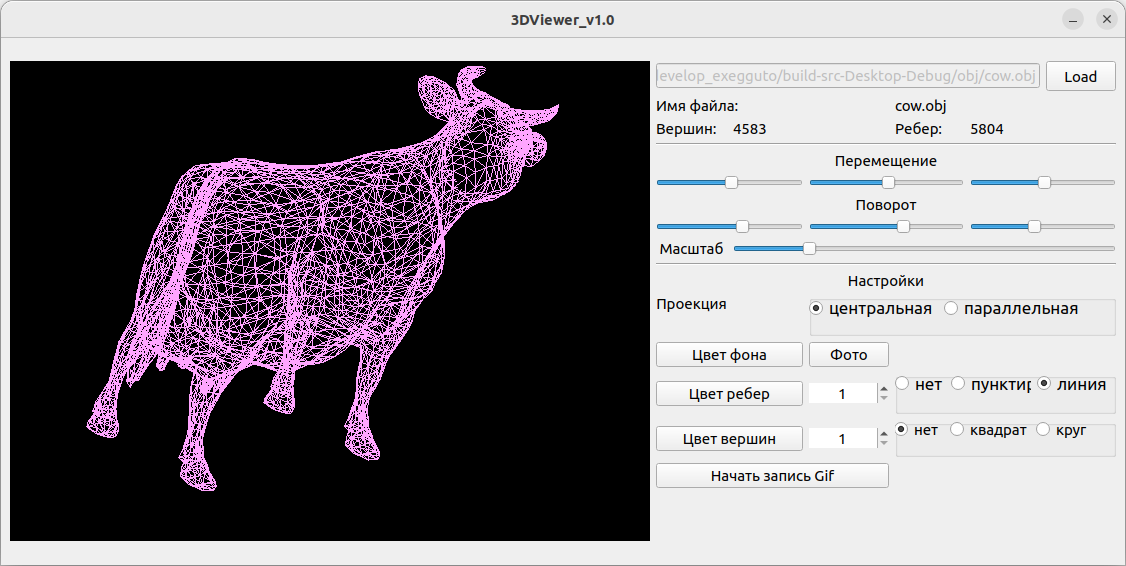
\includegraphics[width=10cm, keepaspectratio]{3dv_affine}

\subsection{Adjustment \& rendering zone}

This is where the magic happens. You can instantly change the color of edges, nodes and background by pressing the corresponding button
and then selecting the color you want in the opened window. The spinboxes in the second column adjust edges' width and nodes' radius.

\vspace{0.5cm}

There are 3 sets of radio buttons in here:

\begin{enumerate}
    \item The one at the top to change the projection
    \item The one in the middle to change the way edges are displayed
    \item The one at the bottom to change the way nodes are displayed
\end{enumerate}

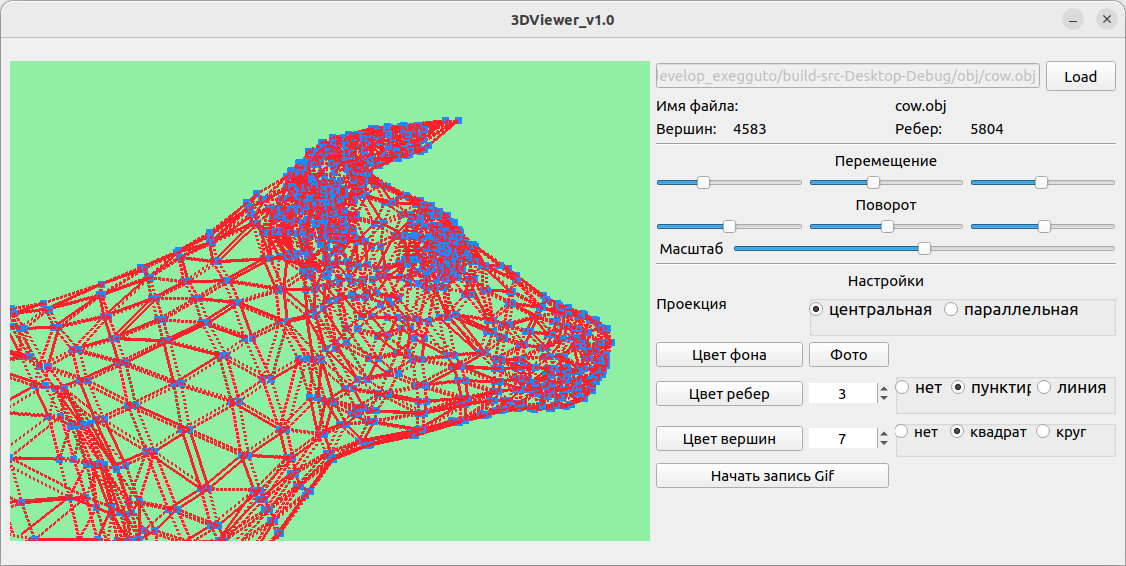
\includegraphics[width=10cm, keepaspectratio]{3dv_coloursandstuff}

\vspace{0.5cm}

There are also two more buttons:

\begin{enumerate}
    \item To save currently displayed image in either \textit{.jpg} or \textit{.bmp} format
    \item To capture next 5 seconds of the image (feel free to manipulate it during this time) and render them into a \textit{.gif} image 
\end{enumerate}

\pagebreak

\section{Conclusion}

Well, this about sums it all up. If you actually managed to read through all of this nonsense all the way down here,
we wish you all the best and hope you have an above-average day.
\end{document}
